% Definicoes do \documentclass

\documentclass[ppginf, pep]{esinucpel}

\usepackage[utf8]{inputenc}
\usepackage[T1]{fontenc}
\usepackage{graphicx}
\usepackage{float}
% \usepackage{caption}
% \usepackage{hyperref}
\usepackage{url}
\usepackage{listings}
\usepackage{color}
\usepackage{lscape}
\usepackage{scrextend}
\usepackage{dirtree}
% \usepackage{listingsutf8}
% \lstset{inputencoding=utf8/latin1}

\graphicspath{ {images/} }
% \captionsetup{compatibility=false}

\renewcommand{\baselinestretch}{1.5}

% Code blocks
\definecolor{dkgreen}{rgb}{0,0.6,0}
\definecolor{gray}{rgb}{0.5,0.5,0.5}
\definecolor{mauve}{rgb}{0.58,0,0.82}
\definecolor{lightgray}{rgb}{.9,.9,.9}
\definecolor{darkgray}{rgb}{.4,.4,.4}
\definecolor{purple}{rgb}{0.65, 0.12, 0.82}
\lstdefinelanguage{JavaScript}{
  keywords={break, case, catch, continue, debugger, default, delete, do, else, false, finally, for, function, if, in, instanceof, new, null, return, switch, this, throw, true, try, typeof, var, void, while, with, async, await, let, const},
  morecomment=[l]{//},
  morecomment=[s]{/*}{*/},
  morestring=[b]',
  morestring=[b]",
  morestring=[b]`,
  ndkeywords={class, export, boolean, throw, implements, import, this},
  keywordstyle=\color{blue}\bfseries,
  ndkeywordstyle=\color{darkgray}\bfseries,
  identifierstyle=\color{black},
  commentstyle=\color{purple}\ttfamily,
  stringstyle=\color{red}\ttfamily,
  sensitive=true
}

\lstset{frame=tb,
  language=JavaScript,
  aboveskip=3mm,
  belowskip=3mm,
  showstringspaces=false,
  columns=flexible,
  basicstyle={\small\ttfamily},
  numbers=none,
  numberstyle=\tiny\color{gray},
  keywordstyle=\color{blue},
  commentstyle=\color{dkgreen},
  stringstyle=\color{mauve},
  breaklines=true,
  breakatwhitespace=true,
  tabsize=4
}

% Inline code
\newcommand{\code}[1]{\texttt{#1}}



%\usepackage[acronym]{glossaries}

% Abreviaturas:
%\newacronym{tc39}{TC39}{Technical Committee 39}

\title{Harmonic: Gerador de Sites Estáticos}

\author{Matté}{Fabrício da Silva}
\advisor[Prof.]{Rodrigues}{Sérgio Luis}
% \coadvisor[Prof.~Dr.]{Aguiar}{Marilton Sanchotene de}
% \collaborator[Prof.~Dr.]{Aguiar}{Marilton Sanchotene de}


\keyword{Gerador de Sites Estáticos}
\keyword{Node.js}
\keyword{ECMAScript 2015}

%\makeglossaries
\begin{document}

%\renewcommand{\advisorname}{Orientadora}           %descomente caso tenhas orientadora
%\renewcommand{\coadvisorname}{Co-orientadora}      %descomente caso tenhas co-orientadora

\maketitle
\sloppy

\newpage

% Folha de Rosto
\begin{center}
    \large{\textbf{Fabrício da Silva Matté}}
    
    \vspace{8cm}
    
    \LARGE{\textbf{Harmonic: Gerador de Sites Estáticos}}
\end{center}

\vspace{1cm}

\begin{addmargin}[8cm]{0cm}
Trabalho de Conclusão de Curso para obtenção do título de bacharel em Tecnologia em Sistemas para Internet, do Instituto Federal Sul-rio-grandense.
\vspace{5pt}\\Orientador: Prof. Sérgio Luis Rodrigues
\end{addmargin}

\vspace{6cm}
\begin{center}
\large{Pelotas
\\2016}
\end{center}


% Glossário de abreviaturas
%\printglossary[type=\acronymtype,title=Lista de abreviaturas e siglas]

% Sumário
\tableofcontents

\listoffigures

\listoftables

\begin{listofabbrv}{Harmonic}
    \item[CLI] Command-line interface
    \item[CMS] Content Management System
    \item[JSON] JavaScript Object Notation
    \item[HTML] HyperText Markup Language
    \item[HTTP] Hypertext Transfer Protocol
    \item[NVM] Node Version Manager
    \item[PHP] PHP: Hypertext Preprocessor
    \item[RF] Requisito Funcional
    \item[RNF] Requisito Não-Funcional
    \item[TC39] Technical Committee 39
    \item[RSS] Rich Site Summary
\end{listofabbrv}

% Resumo em Portugues (no maximo 250 palavras)
\begin{abstract}
\setstretch{1.0}

O projeto Harmonic tem por objetivo desenvolver um gerador de sites estáticos, utilizando como base a plataforma Node.js juntamente com os recursos mais recentes da linguagem JavaScript que foram especificados no padrão ECMAScript 2015 \cite{es2015}, o qual foi finalizado e oficializado como padrão da linguagem JavaScript em meados de junho de 2015. O compilador Babel é utilizado para atingir este objetivo, o qual transforma código que utiliza recursos de especificações recentes e futuras do JavaScript em código que pode ser executado nos motores JavaScript atuais.

O Harmonic roda sobre a plataforma Node.js, que é, de forma resumida, um motor JavaScript combinado com servidor Web, que permite execução do mesmo código JavaScript em todas as principais plataformas (Windows, Linux e Mac), sem possuir as restrições de segurança comumente encontradas no ambiente de navegadores. Ou seja, o código JavaScript executado pelo Node.js tem acesso completo ao sistema de arquivos e rede da máquina hospedeira, e esta é uma das principais capacidades do Node.js das quais o Harmonic utiliza para gerar sites estáticos.

\end{abstract}

\begin{englishabstract}{Harmonic: Static Site Generator}{Static Site Generator, Node.js, ECMAScript 2015}
\setstretch{1.0}

The Harmonic project aims to develop a static site generator, using the Node.js platform as its base together with the most recent JavaScript features that have been specified in the ECMAScript 2015 standard \cite{es2015}, which was completed and officially published as the JavaScript language standard in mid-June 2015. The Babel compiler is utilized to achieve this goal, which transforms code that uses features from the most recent and future JavaScript specifications into code that can be run in the current JavaScript engines.

Harmonic runs on the Node.js platform, which is, basically, a JavaScript engine combined with a Web server, which enables the same JavaScript code to run in all the major platforms (Windows, Linux and Mac), having none of the security restrictions often found in the browser environment. That is, the JavaScript code run by Node.js has full access to the host machine's file system and network, and this is one of the main Node.js capabilities of which Harmonic uses to generate static sites.

\end{englishabstract}

\chapter{Introdução}

Ao se construir um site depara-se com inúmeros problemas como, por exemplo, como resolver as partes de \textit{layout} que são repetidas em várias páginas do projeto, outro desafio é como entregar o projeto para o cliente: não seria viável realizar o projeto com um conjunto de tecnologias específicas, como por exemplo PHP (\textit{PHP: Hypertext Preprocessor}) e MySQL, para entregar para um cliente que trabalha com um conjunto de tecnologias incompatíveis.
Portanto, comumente usa-se uma ferramenta como o \code{wget} para percorrer o projeto e transformar as páginas em HTML estático. Embora seja possível automatizar este processo, não seria a solução ideal. Seria necessário algo mais eficaz para suprir essa necessidade. A partir desta carência, surgem então ferramentas próprias para a criação de sites estáticos \cite{tableless}.


Na perspectiva de suprir essas funcionalidades surge a proposta desse trabalho  denominado Harmonic que é um gerador de sites estáticos. A ideia é que o usuário crie páginas e até mesmo um blog de forma estática, usando apenas  Markdown para formatação de textos e posts. 

O projeto Harmonic, é um programa capaz de gerar uma estrutura de pastas e \emph{arquivos fonte} onde o usuário pode criar e gerenciar o conteúdo de seu site, além de poder instalar, criar ou personalizar \emph{temas}, que são grupos de arquivos de \textit{template}.

O Harmonic pode ser instalado de forma gratuita pelo gerenciador de pacotes \emph{npm} \cite{npm}. Os temas do Harmonic geralmente são disponibilizados através de pacotes também distribuídos pelo npm, mas o usuário também possui a opção de criar temas privados sem a necessidade de publicá-los no npm, assim como não compartilhá-los com o público.

Outra característica importante do projeto Harmonic é que todo o seu desenvolvimento é de forma aberta, tendo o seu \emph{código fonte} acessível em um repositório hospedado no serviço do GitHub \cite{github}, assim como todas as discussões, reportagens de problemas, tomadas de decisões e governança do projeto ocorre de forma aberta no próprio \textit{issue tracking system} do GitHub, que é utilizado como uma espécie de sistema de gerenciamento do projeto.

O projeto Harmonic está sendo desenvolvido sobre a plataforma \emph{Node.js}, que possibilita a execução de programas escritos na linguagem de programação JavaScript nos principais Sistemas Operacionais (Windows, Linux e Mac). Desta forma, todo projeto é escrito em uma linguagem de programação simples de escrever e contribuir, além de não possuir limitações comumente encontradas no ambiente de um navegador.

O Harmonic conta com uma CLI (\textit{Command-line interface}), ou seja, todos os seus recursos e comandos são acessados através da linha de comando, utilizando programas como o \textit{Command Prompt} no Windows, ou o Terminal no Linux ou no OS X. Isto facilita a implementação de rotinas de automação envolvendo o Harmonic, seguindo o padrão imposto por este gênero de software que sempre conta com uma interface de linha comando. As interfaces de linha de comando também são muito mais leves que interfaces gráficas, pois não alocam recursos, como por exemplo memória e CPU, do sistema operacional para exibir janelas e componentes de interface. Usuários avançados muitas vezes preferem usar interfaces de linha de comando ao invés de interfaces gráficas, pois são mais fácil no sentindo em que todas as ações são realizadas com uma linha de texto, invés de clicar através de sequências de menus, submenus, campos de entrada e botões.

% O foco principal deste projeto está na ergonomia do usuário e simplicidade de ser utilizado. O usuário está sempre em primeiro plano. Recursos como recompilar arquivos automaticamente ao serem modificados assim como recarregar o site em desenvolvimento automaticamente quando há mudanças, além da excelente performance da ferramenta e a simplicidade da interface de linha de comando, facilitam a vida do usuário e o deixam mais produtivo.

% Um dos objetivos complementares deste projeto é aprender, explorar e demonstrar os novos recursos oferecidos pela linguagem JavaScript, como aqueles introduzidos nas novas edições da especificação ECMAScript, assim como nas propostas que estão em andamento no processo de padronização do TC39 (Technical Committee 39, grupo responsável pela evolução da linguagem JavaScript) da associação \textit{ECMA International}. % TODO: TC39 provavelmente deveria ser marcado como acrônimo

Este trabalho é dividido da seguinte forma nos capítulos que compõem esse trabalho: fundamentação teórica, metodologia de pesquisa, modelagem do sistema, tecnologias e ferramentas utilizadas, descrição do sistema e considerações finais. Na seção 1.1, 1.2 e 1.3 deste capítulo é descrito a justificativa, os objetivos e o contexto de pesquisa respectivamente.

\section{Justificativa}

A partir de pesquisas e estudos com ferramentas similares, notou-se que muitos dos sistemas semelhantes são difíceis de instalar, não suportam certos sistemas operacionais como Windows, possuem configurações complexas ou são muito complicados de utilizar. Assim, constatou-se a necessidade de um gerador de sites estáticos multiplataforma, eficiente e prático.

Na proposta deste trabalho, entende-se como multiplataforma os sistemas que sejam compatíveis com a mais ampla gama de sistemas operacionais, independente de \textit{hardware}. Bem como, sistemas eficientes são aqueles que utilizam relativamente pouca memória e concluem o processamento em tempo apropriado. Como sistemas práticos, entende-se que necessitam de poucos comandos cuja sua sintaxe é extremamente simples, desde a criação até a execução de um site.

Um aprofundamento sobre a pesquisa dos sistemas semelhantes é debatido na seção 3.1.

\section{Objetivos}

O objetivo principal deste trabalho é explorar a área de geradores de sites estáticos, criando uma nova ferramenta de geração de sites estáticos multiplataforma, eficiente, fácil de instalar, com o mínimo de complexidade para criar e executar um site estático.

Outro objetivo do projeto Harmonic é explorar ao máximo os novos recursos e propostas do ECMAScript, o padrão oficial da linguagem JavaScript. O próprio nome Harmonic é derivado deste objetivo, uma vez que o processo atual de evolução do padrão ECMAScript foi nomeado Harmony pelo criador da linguagem JavaScript, Brendan Eich \cite{harmony}.

\section{Contexto de Pesquisa}

O contexto de pesquisa dessa monografia foi iniciado pelos autores Jaydson Gomes \cite{jaydson} e Átila Fassina \cite{atila}, juntamente com a organização JS Rocks \cite{jsrocks} (antigamente chamada de ES6 Rocks).

Em 2014, o autor deste trabalho começou a contribuir para os esforços desta equipe dando continuidade ao projeto Harmonic. Atualmente, atuo como um dos líderes do projeto, onde faço parte da direção avaliando contribuições e conduzindo o projeto.

O Harmonic é um projeto de código fonte aberto disponível no GitHub. Além de contribuições de membros da organização interna JS Rocks, o projeto também aceita contribuições de pessoas e organizações externas as quais serão avaliadas pelos mantenedores oficiais do projeto.

\chapter{Fundamentação Teórica}

A proposta dos sites estáticos é um tema bem popular atualmente, tendo mais de 435 geradores de sites estáticos já existentes e que vem aumentando a cada ano, conforme \textit{Static Site Generators} \cite{staticsitegenerators}.

Ao contrário dos sites dinâmicos, que requisitam banco de dados e executam lógica no servidor para cada requisição, todo o conteúdo de um site estático é gerado instantaneamente antes de qualquer acesso por parte de usuários, assim podendo ser hospedado em um servidor que não necessita de banco de dados nem suporte a nenhuma linguagem de programação.

Além disto, como diz David Walsh \cite{dwb}, sites estáticos são muito mais rápidos que os dinâmicos, pois todo processamento de conteúdo já foi realizado no momento da geração do site estático e não a cada requisição como nos sites dinâmicos. Outro ponto é a segurança: sites estáticos são mais seguros que os dinâmicos pois não possuem lógica de programação no servidor, assim eliminando falhas na programação no lado do servidor.

Foi então realizado um estudo visando as principais características e diferenças entre sites estáticos e dinâmicos, culminando na tabela comparativa \ref{table:comparacao_sites}.

\begin{table}[H]
    \centering
    \setstretch{1.0}
    \caption{Comparação entre sites estáticos e dinâmicos.}
    \vspace{5pt}
    \small
    \begin{tabular}{ | p{7cm} | p{3.5cm} | p{3.5cm} |}
    \hline
    & \textbf{Sites estáticos} & \textbf{Sites dinâmicos} \\ \hline
    Páginas são servidas diretamente do disco para a rede & Sim & Não \\ \hline
    Conseguem buscar páginas inteiramente do cache do navegador & Sim & Não \\ \hline
    Necessitam de banco de dados instalado no servidor & Não & Sim \\ \hline
    Necessitam de uma linguagem de programação instalada e configurada no servidor & Não & Sim \\ \hline
    Executam lógica de programação no servidor, podendo haver falha de segurança e permitindo invasão \textit{hacker} & Não & Sim \\ \hline
    São gerenciáveis & Sim, através de um gerador de sites estáticos & Sim, através de um CMS (\textit{Content Management System}) \\ \hline
    
    % Harmonic & Linux, OS X e Windows. & Node.js & Posts, páginas, rascunhos, templates personalizados, permalinks, internacionalização. Suporta o formato Markdown. & Sim & Sim & Trabalho futuro & Sim \\
    % \hline
    \end{tabular}
    \normalsize
    \vspace{5pt}
    \\Fonte: Elaborado pelo autor.
    \label{table:comparacao_sites}
\end{table}

A partir dos dados da tabela \ref{table:comparacao_sites}, percebe-se que sites estáticos possuem uma proposta atraente não somente em termos de desempenho e segurança, mas também em termos de custos. Já que sites não necessitam de suporte a qualquer linguagem de programação nem banco de dados no servidor, os custos de hospedagem de sites estáticos são muito mais baixos. Existem até mesmo hospedagens gratuitas e de qualidade que garantem a confiabilidade para os usuários acessarem sites estáticos, como o GitHub Pages \cite{github_pages}, que realmente são completamente gratuitas e não adicionam qualquer tipo de propaganda ao seu site.

Praticamente todos geradores de sites suportam a escrita de conteúdo através da linguagem de marcação Markdown, que é basicamente uma versão simplificada, mais fácil de escrever e ler do que a linguagem de marcação HTML (\textit{HyperText Markup Language}). Markdown é uma ferramenta de conversão de texto para HTML para escritores Web \cite{markdown}. O projeto Harmonic também suporta a linguagem de marcação Markdown e o converte para HTML no momento da geração do conteúdo.

O projeto Harmonic é desenvolvido sobre a plataforma Node.js, que suporta todos os principais sistemas operacionais (OS X, Linux, Solaris, FreeBSD, OpenBSD, Windows) o que permite executar o mesmo código em todas estas plataformas. A plataforma Node.js executa código JavaScript, que é uma linguagem de programação leve e bem simplificada \cite{mdn_js_intro}, assim facilitando no desenvolvimento. O Node.js também possui mais de 250.000 pacotes públicos publicados no registro de pacotes mais popular, npm \cite{npm}, o que torna o desenvolvimento muito mais ágil permitindo reutilizar "blocos de construção"~ para construir sistemas mais elaborados \cite{micromodules}.

\chapter{Metodologia de Pesquisa}

A ideia do projeto surgiu para criar uma nova forma diferente de criar sites, fora do usual que são os sites dinâmicos, os quais possuem banco de dados, programação no servidor. % TODO descrever

Através da participação na comunidade JavaScript, surgiu a ideia de criar um gerador de sites estáticos, que oferecesse uma forma mais simples, eficiente e prática de criar sites estáticos.


\section{Sistemas Semelhantes}

Foram examinados diversos sistemas semelhantes no início deste projeto, e assim foi constatada a falta de um sistema compatível com todos os principais sistemas operacionais, fácil de instalar e prático que não necessite da instalação de \textit{plugins} para funcionalidades básicas que um usuário normalmente espera de um gerador de sites estáticos.

Foram avaliados os seguintes projetos: Jekyll \cite{jekyll}, Metalsmith \cite{metalsmith}, Hugo \cite{hugo}, Hexo \cite{hexo}. Nessa avaliação foram observadas várias características como: sistemas operacionais suportados, em qual linguagem de programação foi desenvolvido, que recursos são oferecidos aos usuários, se atualiza o navegador automaticamente ao recompilar o site estático, e como última característica se o código fonte é aberto.

Conforme pode ser observado na tabela \ref{table:comparacao_sistemas}, alguns trabalhos semelhantes possuem características em comum, contudo com a pesquisa destes foi possível conhecer um pouco sobre a área de gerador de sites estáticos, seus objetivos e desafios a serem superados. O estudo desses sistemas semelhantes foi fundamental para elaboração desta monografia.

Note que o Jekyll não suporta o sistema operacional Windows oficialmente, portanto usuários de Windows enfrentam uma grande dificuldade para utilizá-lo. Já o Metalsmith é multi-plataforma e extremamente poderoso, mas não oferece funcionalidades caso o usuário não instale e configure os \textit{plugins} desejados, o que o torna desnecessariamente complexo para os casos de uso mais simples.

O principal diferencial do Harmonic é sua praticidade. O Harmonic pode ser facilmente instalado em qualquer um dos principais sistema operacionais, o usuário precisa de apenas dois comandos para criar e executar um site estático, e o Harmonic já conta com todos os recursos essenciais para o gerenciamento do site estático sem necessitar de configurações extras nem instalações de \textit{plugins}.

\begin{landscape}
    \begin{table}[H]
        \centering
        \setstretch{1.0}
        \caption{Comparação entre sistemas semelhantes.}
        \vspace{5pt}
        \small
        \begin{tabular}{ | p{2cm} | p{3.5cm} | l | p{7.5cm} | p{1.6cm} | p{2cm} | p{1.5cm} | p{1.3cm} |}
        \hline
        Projeto & Sistemas Operacionais & Escrito em & Recursos & Recompila automaticamente & Atualiza o navegador automaticamente ao recompilar & \textit{plugins} & Código fonte aberto \\ \hline
        Jekyll & Linux, Unix e OS X. Windows não é suportado oficialmente. & Ruby & Posts, páginas, categorias, permalinks, templates personalizados. Suporta os formatos Markdown, Textile e Liquid. & Sim & Não & Sim & Sim \\ \hline
        Metalsmith & Suporta praticamente todas plataformas, embora alguns \textit{plugins} possam não ter suporte a todas as plataformas. & Node.js & Serve como uma abstração para manipulação de arquivos e diretórios, logo não suporta nenhum recurso nativamente e todas as funcionalidades se dão através de \textit{plugins}. & Sim, através de \textit{plugins} & Sim, através de \textit{plugins} & Sim & Sim \\ \hline
        Hugo & Linux, OS X e Windows. & Go & Páginas, templates personalizados, seções, ordenação de conteúdo, permalinks, pretty URLs, aliases (redirecionamentos), geração automática e personalizada de sumários, shortcodes, tempo de leitura, contagem de palavras. Suporta o formato Markdown além de outros formatos através de \textit{plugins}. & Sim & Sim & Sim & Sim \\ \hline
        Hexo & Linux, OS X e Windows. & Node.js & Posts, páginas, rascunhos, templates personalizados, permalinks, helpers, internacionalização, integração de  serviços de deploy. Suporta o formato Markdown. & Sim & Sim, através de \textit{plugins} & Sim & Sim \\
        \hline
        Harmonic & Linux, OS X e Windows. & Node.js & Posts, páginas, rascunhos, templates personalizados, permalinks, internacionalização. Suporta o formato Markdown. & Sim & Sim & Trabalho futuro & Sim \\
        \hline
        \end{tabular}
        \normalsize
        \vspace{5pt}
        \\Fonte: Elaborado pelo autor.
        \label{table:comparacao_sistemas}
    \end{table}
\end{landscape}

\chapter{Modelagem do Sistema}

Após especificar o que o sistema poderia oferecer ao seus usuários, passou-se à etapa de criação dos diagramas para identificar como deve ser o processo de comunicação entre os vários componentes do sistema e a utilização do UML facilitou a modelagem do software.

UML é uma linguagem de modelagem que auxilia os desenvolvedores na montagem dos requisitos e do comportamento dos processos no sistema, também atua na descoberta de possíveis necessidades físicas que possam surgir na implementação de uma determinada ferramenta \cite{uml}.

UML é uma metodologia que disponibiliza diversas maneiras para analisar uma determinada questão e neste projeto será utilizado uma abordagem orientada a objetos, que auxilia na reutilização de métodos ou atributos, melhorando o desenvolvimento e a manutenção do sistema. A seção 4.1 apresenta um diagrama de sequência, a seção 4.2 apresenta o diagrama de casos de uso, e a seção 4.3 apresenta o diagrama de classes.

% Quebra de página para manter o gráfico junto com o texto
\newpage
\section{Diagrama de Sequência}

Foram criados diagramas de sequência pois estes ajudam a planejar o fluxo de informações e operações a serem realizadas pelas rotinas do sistema. O diagrama de sequência da execução do site estático, que é uma das principais funcionalidades do Harmonic, pode ser conferido na figura \ref{fig:sequencia}.

\begin{figure}[H]
    \centering
    \caption{Diagrama de sequência da execução de um site estático do Harmonic.}
    \vspace{5pt}
    \includegraphics[width=\textwidth]{sequencia}
    \\Fonte: Elaborado pelo autor.
    \label{fig:sequencia}
\end{figure}

% Quebra de página para manter o gráfico junto com o texto
% \newpage
\section{Diagrama de Casos de Uso}

Foi criado um diagrama de casos de uso pois este facilita mapear as funcionalidades que o sistema deve desempenhar assim como as relações entre elas. O diagrama de casos de uso do Harmonic pode ser conferido na figura \ref{fig:casos_de_uso}.

\begin{figure}[H]
    \centering
    \caption{Diagrama de casos de uso do Harmonic.}
    \vspace{5pt}
    \includegraphics[width=\textwidth]{casos-de-uso}
    \\Fonte: Elaborado pelo autor.
    \label{fig:casos_de_uso}
\end{figure}

\section{Diagrama de Classes}

Segundo Guedes, o diagrama de classes define a estrutura das classes utilizadas pelo sistema, determinando seus atributos e métodos, e também estabelece as relações
e trocas de informações entre as classes do sistema \cite{uml}.

Assim sendo, foi elaborado um diagrama de classes que exibe as principais classes do Harmonic e a comunicação entre elas. Entre elas estão a classe  \textit{Harmonic} que encapsula todas as funcionalidades principais do projeto Harmonic, a classe  \textit{Helper} que possui várias funções utilitárias utilizadas pela classe  \textit{Harmonic}, a classe \textit{Theme} que encapsula o manuseio de arquivos de um determinado tema, a classe \textit{MissingFileError} que é uma especialização da classe nativa \textit{Error} e serve para comunicar um erro devido a ausência de arquivos essenciais durante uma dada operação, como por exemplo a falta do arquivo de configuração \code{harmonic.json} caso o mesmo tenha sido excluído ou caso não existe um site estático do Harmonic onde o comando foi executado, e também a classe \textit{CLI\_Program} que representa todas as possíveis interações com a interface de linha de comando do Harmonic. O diagrama de classes do Harmonic pode ser visto na figura \ref{fig:classes}.

\begin{figure}[htbp]
    \centering
    \caption{Diagrama de classes do Harmonic.}
    \vspace{5pt}
    \hspace*{-1.5cm}
    \includegraphics[width=1.2\textwidth]{classes}
    \\Fonte: Elaborado pelo autor.
    \label{fig:classes}
\end{figure}

Um dos principais métodos da classe Harmonic é o \code{generateFiles}, cujo código fonte pode ser visto na figura \ref{fig:code_generateFiles}. O método \code{generateFiles} da classe Harmonic é responsável pelo processamento e geração dos arquivos de \textit{posts} e páginas do site estático. Este método recebe dois parâmetros como entrada, \code{files} e \code{fileType}. O parâmetro \code{fileType} determina o tipo de conteúdo a ser gerado, sendo ele \code{post} para \textit{posts} ou \code{page} para páginas. O parâmetro \code{files} é um objeto cujas propriedades são as linguagens suportadas pelo site estático e seus valores são os caminhos para os arquivos fontes do tipo de conteúdo a ser gerado na respectiva linguagem.

Este método realiza o \textit{parsing} do cabeçalho de meta-informações do conteúdo (\textit{post} ou página), trata para não publicar conteúdos ocultos nem conteúdos agendados para o futuro, processa o conteúdo Markdown transformando-o em HTML, combina-o com o \textit{template} do tema ativo e escreve os arquivos HTML gerados no caminho de saída, como especificado no arquivo de configuração \code{harmonic.json}. Então, o método retorna informações sobre os conteúdos gerados de forma propriamente ordenada para que estes sejam utilizados na geração da página inicial e das listagens de \textit{posts} por categoria.

Este método também demonstra o objetivo do Harmonic de explorar os novos recursos e propostas da linguagem JavaScript. O método em si é uma \textit{Async Function}, um novo recurso da linguagem que facilita o controle de fluxo de execução assíncrono utilizando a palavra-chave \code{await}. As \textit{Async Functions} foram aceitas como parte do padrão ECMAScript em julho de 2016, já sendo incorporadas ao último rascunho da especificação e esperadas a serem publicadas como parte da próxima edição oficial da especificação, o ECMAScript 2017 \cite{es_finished_proposals}. O método também são utilizados recursos experimentais que ainda estão tramitando no processo de desenvolvimento, como a proposta \textit{Function Bind Syntax} (utilizando o operador \code{::}), além de várias outras funcionalidades padronizadas recentemente, como constantes, \textit{Arrow Functions} e \textit{Template Literals}, que foram padronizadas na edição ECMAScript 2015.

\begin{figure}[htbp]
    \centering
    \caption{Código fonte do método \code{generateFiles} da classe Harmonic.}
    \vspace{5pt}
    \lstset{language=JavaScript}
    \begin{lstlisting}
async generateFiles(files, fileType) {
    const langs = Object.keys(files);
    const config = this.config;
    const generatedFiles = {};
    const currentDate = new Date();
    const tokens = config.header_tokens || ['<!--', '-->'];
    const metadataDefaults = {
        layout: fileType
    };

    const filesPath = fileType === 'post' ? postspath : pagespath;

    await Promise.all([].concat(...langs.map((lang) => files[lang].map(async (file) => {
        const md = new MkMeta(path.join(this.sitePath, filesPath, lang, file));
        md.defineTokens(tokens[0], tokens[1]);

        const metadata = this.normalizeMetaData(md.metadata(), metadataDefaults);
        metadata.content = new nunjucks.runtime.SafeString(md.markdown({
            crop: '<!--more-->'
        }));

        const template = this.getTemplate(metadata.layout);
        const filename = getFileName(file);
        const permalink = fileType === 'post' ? config.posts_permalink : config.pages_permalink;

        const filePath = permalinks({
            replacements: [{
                pattern: ':year',
                replacement: metadata.date.getFullYear()
            }, {
                pattern: ':month',
                replacement: (metadata.date.getMonth() + 1)::padStart(2, '0')
            }, {
                pattern: ':title',
                replacement: filename
            }, {
                pattern: ':language',
                replacement: lang
            }],
            structure: getStructure(config.i18n.default, lang, permalink)
        });
    \end{lstlisting}
    \label{fig:code_generateFiles}
\end{figure}
\begin{figure}[htbp]%\ContinuedFloat
    \centering
    \begin{lstlisting}
        metadata.file = filesPath + file;
        metadata.filename = filename;
        metadata.link = filePath;
        metadata.lang = lang;

        const contentHTMLFile = template
            .render({
                [fileType]: {
                    content: new nunjucks.runtime.SafeString(md.markdown()),
                    metadata
                },
                config,
                lang
            })
            .replace(/<!--[\s\S]*?-->/g, '');

        if(fileType === 'page') {
            metadata.content = new nunjucks.runtime.SafeString(contentHTMLFile);
        }

        if (metadata.published && metadata.published === 'false') {
            return;
        }

        if (metadata.date && metadata.date > currentDate) {
            console.log(clc.info(`Skipping future ${fileType} ${metadata.filename}`));
            return;
        }

        const publicFileDirPath = path.join(this.sitePath, 'public', filePath);
        const publicFilePath = path.join(publicFileDirPath, 'index.html');
        await mkdirpAsync(publicFileDirPath);

        await fs.writeFileAsync(publicFilePath, contentHTMLFile);
        console.log(clc.info(`Successfully generated ${fileType} ${filePath}`));

        generatedFiles[lang] = generatedFiles[lang] || [];
        generatedFiles[lang].push(metadata);
    }))));

    return fileType === 'post' ? this.sortByDate(generatedFiles) : this.sortByName(generatedFiles);
}
    \end{lstlisting}
    Fonte: Elaborado pelo autor.
\end{figure}


\chapter{Tecnologias e Ferramentas Utilizadas}

\section{JavaScript}

JavaScript é uma linguagem de programação orientada a objetos multiplataforma. Dentro de um ambiente hospedeiro (por exemplo, um navegador web), JavaScript pode ser conectado aos objetos de seu ambiente para prover controle sobre eles. O padrão oficial da linguagem JavaScript é o ECMAScript \cite{mdn_js_intro}.

O JavaScript obteve uma evolução significativa nos últimos anos, tornando-se assim uma linguagem de propósito geral muito utilizada no mundo. Essa por sua vez é mais conhecida como a linguagem incorporada aos navegadores Web, mas também houve um grande crescimento em sua adoção por parte de servidores e aplicações embarcadas \cite{es2015}.

O projeto Harmonic escolheu esta linguagem de programação devido a sua ampla aceitação no mercado e rápida evolução, além de esta linguagem ser relativamente simples e fácil de trabalhar, contendo centenas de milhares de pacotes comunitários que facilitam no desenvolvimento de praticamente qualquer sistema.

\section{Node.js}

Node.js é uma plataforma de código fonte aberto que permite construir aplicações em rede utilizando a linguagem JavaScript. Node.js é construído em cima do V8, uma máquina virtual JavaScript moderna que também é utilizada pelo navagedor Web Google Chrome \cite{instant_nodejs_starter:03}.

Node.js é um \textit{runtime} JavaScript assíncrono orientado a eventos \cite{nodejs}. Isto que dizer que o Node.js pode ser considerado uma plataforma que combina um motor JavaScript com acesso a recursos do sistema operacional hospedeiro.

A plataforma Node.js roda diretamente sobre o sistema operacional, com isto é possível executar código JavaScript completamente fora do ambiente de um navegador Web. Assim sendo, o Node.js não interage com uma página da Web diretamente, mas sim com os recursos do computador hospedeiro. Por exemplo, o Node.js pode receber e realizar requisições HTTP (\textit{Hypertext Transfer Protocol}), ler e escrever no sistema de arquivos, e se comunicar com outros processos, \textit{sockets} e \textit{drivers} do sistema operacional \cite{javaworld}.

Todo o projeto Harmonic é construído sobre a plataforma Node.js, que realiza toda lógica de negócios e leitura e escritas ao sistema de arquivos do usuário.

\section{npm}

O npm é o gerenciador de pacotes padrão da plataforma Node.js, contando com mais de 250.000 pacotes publicados \cite{npm} e provendo mais de um bilhão de instalações de pacotes semanalmente \cite{npm_packages}.

O projeto Harmonic escolheu o npm como sua plataforma de distribuição e gerenciador de dependências devido ao seu fácil acesso, altíssima resiliência e ubiquidade na comunidade Node.js.

\section{JSON}

JSON (\textit{JavaScript Object Notation}) é um formato de troca de informações eficiente. É fácil de ler e escrever manualmente. É fácil de analisar e gerar por computadores, assim como ler e escrever por desenvolvedores \cite{json}.

O projeto Harmonic escolheu o formato JSON para o armazenamento de configurações, pois este formato facilita a operação dos dados tanto pelo sistema quanto pelo usuário final.

\section{Markdown}

Como diz Gruber, o criador desta tecnologia, Markdown é uma ferramenta de conversão de texto para HTML projetada para escritores Web \cite{markdown}. Markdown é uma sintaxe de formatação em texto puro.

O projeto Harmonic escolheu a linguagem Markdown por ser uma linguagem simples e popular, com o intuito de facilitar a autoria de conteúdos.

\section{RSS}

RSS (Rich Site Summary) é um formato para entrega de conteúdo Web que é atualizado regularmente. Sites de notícias, blogs, resultados de pesquisa, e todos estes tipos de sites podem ser concebidos no formato de uma lista de conteúdos frequentemente atualizados. O RSS é um formato utilizado para entregar este conteúdo no formato de uma lista de \textit{links} e dados sobre cada \textit{link} \cite{rss}.

O Harmonic escolheu este formato por ser um padrão aberto bem estabelecido, com o intuito de permitir que usuários possam optar por receber notificações e prévias quando conteúdos novos forem publicados.

\section{gulp}

O gulp é uma sistema de \textit{build} escrito em Node.js. Sua principal função é automatizar tarefas repetitivas e aprimorar a rotina de trabalho. O gulp é composto por um sistema de gerenciamento de tarefas (\textit{Orchestrator}), um formato virtual que descreve um arquivo (\textit{Vinyl}), um adaptador de que converte uma determinada fonte (como o sistema de arquivos do computador) para o formato Vinyl, uma interface de linha de comando e um conjunto de regras para garantir a qualidade de seus \textit{plugins} \cite{gulp}.

O projeto Harmonic escolheu o gulp devido a seu amplo número de \textit{plugins}, grande flexibilidade, simplicidade e desempenho. O Harmonic utiliza o gulp para tarefas de compilação do Babel, verificação de qualidade de código e testes unitários.

\section{Babel}

O Babel é um compilador genérico multi-propósito para JavaScript. Um de seus principais usos é compilar os recursos da próxima geração do JavaScript para ser compatível com os interpretadores atuais \cite{babel}.

O Harmonic escolheu este compilador JavaScript para prover uma maior compatibilidade com as mais diversas versões do Node.js, desde as versões mais antigas, como a versão 0.10, até as mais atuais, como a versão 6. Assim tornando o Harmonic mais resiliente às implementações de novos recursos ou a falta dos mesmos nas diferentes versões do Node.js.

\section{Nunjucks}

Nunjucks é uma linguagem de \textit{templating} sofisticada devolvida pela Mozilla. Os \textit{templates} do Nunjucks suportam vários recursos, entre eles declarações condicionais, laços de repetição, filtros nativos que trabalham com variáveis, herança de \textit{templates} que permite reutilizá-los estendendo e populando outros \textit{templates}, entre outros recursos.

O Nunjucks é parte fundamental da funcionalidade dos temas do Harmonic, pois este provê pontos de inserção nos \textit{templates} do tema para os conteúdos escritos pelo usuário.

% \section{BrowserSync}

\section{Mocha}

O Mocha é um ferramenta de testes unitários, o que permite a automatização de testes de funcionalidades através da escrita de suítes de testes \cite{mocha}.

O autor deste trabalho escolheu esta ferramenta para aumentar a produtividade no desenvolvimento e evitar regressões de erros de programação.

% \section{Travis}

\chapter{Descrição do Sistema}

Neste capítulo será abordado os requerimentos do sistema, assim como a estrutura do projeto completa abordando todos os módulos e detalhando todas suas funcionalidades oferecidas. Finalizando este capítulo, será apresentada uma criação de um site estático simplificado, utilizando os recursos básicos do Harmonic.

\section{Requerimentos do Sistema}

Para instalar o Harmonic, primeiro é necessário possuir o Node.js instalado juntamente com o npm. O Node.js pode ser instalado diretamente pelo seu site <https://nodejs.org>, ou através de vários gerenciadores de pacotes, como o \textit{Advanced Packaging Tool} (apt-get) das distribuições Ubuntu e Debian do Linux, o \textit{Homebrew} do OS X, o \textit{Chocolatey} do Windows, ou programas dedicados para gerenciamento de versões do Node.js, como o n \cite{n} e nvm (Node Version Manager) \cite{nvm}.

A maioria dos métodos de instalação do Node.js já instala o gerenciador de pacotes npm automaticamente por padrão. Caso o usuário não possua o npm instalado após instalar o Node.js, ele pode ser instalado separadamente também como exibido na documentação do npm \cite{npm_fancy_install}, ou compilado a partir de seu código fonte.

Uma vez que o usuário possua a plataforma Node.js e o gerenciador de pacotes npm instalados corretamente, o Harmonic pode ser instalado pelo gerenciador de pacotes npm, através do comando apresentado na figura \ref{fig:install_harmonic}. Este comando é digitado em um programa de linha de comando, como o \textit{Command Prompt} ou \textit{Terminal}.

\begin{figure}[H]
    \centering
    \caption{Instalação do Harmonic.}
    \vspace{5pt}
    \lstset{language=sh}
    \begin{lstlisting}
    npm install -g harmonic
    \end{lstlisting}
    Fonte: Elaborado pelo autor.
    \label{fig:install_harmonic}
\end{figure}

Este comando instala o Harmonic de forma global, ou seja, a interface de linha de comando do Harmonic torna-se disponível em todo sistema.

Note que caso usuário esteja usando o sistema operacional OS X, pode ser necessário consertar as permissões do npm antes de instalar pacotes globais, como é documentado no site do npm \cite{npm_fix_perms}.

\section{Estrutura do Projeto}

O Harmonic divide-se em vários módulos, sendo eles: criação de um site estático, configuração do site estático, criação de \textit{posts}, criação de páginas, geração do site estático, execução do site estático, utilização de temas, além do módulo de ajuda. Na sequência dessa seção será descrito cada módulo.

Assim como a maioria dos pacotes, bibliotecas e ferramentas escritas sobre a plataforma Node.js, o Harmonic está publicado no registro de pacotes do npm e pode ser instalado através do gerenciador de pacotes que faz parte da instalação padrão do Node.js, ou seja, através da ferramenta de linha de comando do npm.

E, similarmente a outros geradores de sites estáticos, o Harmonic conta uma ferramenta de linha de comando que pode ser utilizada para criar um novo site estático, adicionar conteúdo ao mesmo, compilar o site estático e visualizá-lo no navegador.

\section{Módulo de Criação de um Site Estático}

O Harmonic permite a criação de novos sites estáticos através do comando \code{harmonic init}. Este comando gera uma estrutura padrão de pastas e arquivos, onde são guardados todos arquivos fontes do site estático, como pode ser observado na figura \ref{fig:estrutura_harmonic}.

O comando \code{harmonic init} realiza uma série de questionamentos sobre as configurações e personalizações que o site deve possuir (conforme pode ser conferido na figura \ref{fig:harmonic_init}), então escreve estas configurações no arquivo de configuração do site estático \code{harmonic.json}. O usuário pode futuramente modificar estas configurações utilizando o comando \code{harmonic config} ou editando o arquivo de configuração \code{harmonic.json} em qualquer editor de texto, já que o arquivo de configuração é um arquivo de texto no formato \emph{JSON}.

\begin{figure}[H]
    \centering
    \caption{Exemplo do comando "harmonic init".}
    \vspace{5pt}
    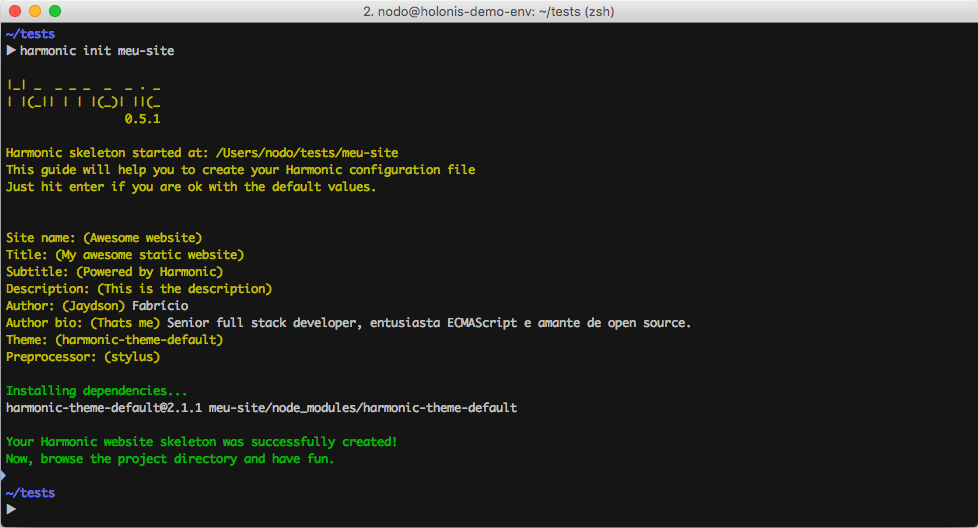
\includegraphics[width=\textwidth]{harmonic_init}
    \\Fonte: Elaborado pelo autor.
    \label{fig:harmonic_init}
\end{figure}

\begin{figure}[H]
    % \centering
    \caption{Estrutura do site estático.}
    \vspace{5pt}
    \dirtree{%
        .1 /.
        .2 harmonic.json\DTcomment{Arquivo de configuração}.
        .2 node\_modules\DTcomment{Pasta onde são instalados os temas}.
        .3 harmonic-theme-default\DTcomment{Tema padrão}.
        .2 package.json\DTcomment{Configuração do pacote, registra as dependências}.
        .2 resources\DTcomment{Arquivos do usuário a serem copiados para o site gerado}.
        .2 src\DTcomment{Pasta onde são criados os arquivos de conteúdo}.
        .3 pages\DTcomment{Arquivos de conteúdo das páginas}.
        .3 posts\DTcomment{Arquivos de conteúdo dos \textit{posts}}.
        .2 public\DTcomment{Site estático gerado}.
    }
    \centering
    Fonte: Elaborado pelo autor.
    \label{fig:estrutura_harmonic}
\end{figure}

\section{Módulo de Configuração do Site Estático}

Após a criação do site estático, a sua estrutura inicial possuirá um arquivo \code{harmonic.json}, onde são armazenadas as configurações escolhidas durante a criação do site. O usuário pode alterar estas configurações através do comando \code{harmonic config}, que irá realizar uma nova série de questionamentos e reconfigurar o site, ou através da edição manual do arquivo de configuração.

Entre as principais configurações de um site estático do Harmonic, estão:

\begin{itemize}
	\item \textbf{\code{title}}: título do seu site que será exibido no navegador.
	\item \textbf{\code{subtitle}}: subtítulo do site. Pode ser utilizado na forma de um \textit{slogan} por alguns temas.
	\item \textbf{\code{description}}: descrição do seu site. Temas podem utilizar esta descrição nas \textit{meta tags} do seu site.
    \item \textbf{\code{domain}}: endereço onde seu site será hospedado. Esta configuração será utilizada no gerador de RSS (\textit{Rich Site Summary}), e pode ser utilizada por alguns temas também.
    \item \textbf{\code{theme}}: nome do tema selecionado.
    \item \textbf{\code{preprocessor}}: Preprocessador CSS padrão a ser utilizado na geração do site estático, caso o tema selecionado não especifique um preprocessador CSS.
    \item \textbf{\code{posts\_permalink}}: Formato da URL dos \textit{posts} gerados, por exemplo \code{:language/:year/:month/:title}. O usuário pode personalizar as URLs dos \textit{posts} utilizando os seguintes parâmetros especiais:
        \subitem \textbf{\code{:language}}: linguagem em que o \textit{post} foi escrito.
        \subitem \textbf{\code{:year}}: ano em que o \textit{post} foi escrito.
        \subitem \textbf{\code{:month}}: mês em que o \textit{post} foi escrito.
        \subitem \textbf{\code{:title}}: título do \textit{post}.
    \item \textbf{\code{pages\_permalink}}: Formato da URL das páginas geradas, por exemplo \code{:language/pages/:title}. Aceita os mesmos parâmetros especiais dos \textit{posts}.
    \item \textbf{\code{index\_posts}}: número de \textit{posts} a serem exibidos na página inicial do site. A forma de paginação depende do tema instalado.
    \item \textbf{\code{i18n}}: é um objeto contendo as seguintes propriedades de internalização:
        \subitem \textbf{\code{languages}}: um \code{array} de linguagens em que o site está disponível. Os comandos de criação de \textit{posts} e páginas criarão um arquivo de conteúdo para cada linguagem dentro da estrutura fonte do site.
        \subitem \textbf{\code{default}}: linguagem padrão do site. A página raiz do site abrirá nesta linguagem, e as postagens e páginas desta linguagem serão geradas sem o segmento \code{:language} em suas URLs.
\end{itemize}

\section{Módulo de Criação de \textit{Posts}}

O usuário pode criar novos \textit{posts} utilizando o comando \code{harmonic new\_post "\textless TÍTULO DO POST\textgreater"}, que criará um arquivo \emph{Markdown} dentro da pasta fonte de \textit{posts} de cada linguagem que o site estático suporta.

Cada \textit{post} criado é automaticamente adicionado às listagens de \textit{posts} da página inicial e de cada categoria a qual pertence em ordem cronológica inversa (\textit{posts} mais recentes são exibidos primeiro).

\subsection{Meta-informações e configurações de \textit{posts}}

Cada arquivo fonte de \textit{post} possui um cabeçalho de meta-informações, no formato de um comentário HTML contendo pares de chaves e valores, como pode ser visto na figura \ref{fig:post_header}.

\begin{figure}[htbp]
    \centering
    \caption{Exemplo de cabeçalho de meta-informações de um \textit{post} do Harmonic.}
    
    \lstset{language=HTML}
    \begin{lstlisting}
    <!--
    layout: post
    title: JavaScript iterables and iterators
    date: 2015-09-15T04:06:02.428Z
    comments: true
    published: true
    keywords: iterables, iterators, ES2015
    description: Understanding JavaScript ES2015 Iterables and Iterators
    categories: iterables, iterators, ES2015, articles
    authorName: UltCombo
    authorLink: https://twitter.com/Ult_Combo
    authorDescription: Full Stack developer, ECMAScript enthusiast, open source lover.
    authorPicture: https://s.gravatar.com/avatar/326fba1c2980ce0073f6b212acf71ea0
    -->
    \end{lstlisting}
    
    Fonte: Elaborado pelo autor.
    \label{fig:post_header}
\end{figure}

As meta-informações e configurações de \textit{posts} disponíveis são:

\begin{itemize}
	\item \textbf{\code{layout}}: nome do arquivo HTML do tema selecionado a ser utilizado na renderização deste \textit{post}. O valor padrão é \code{post}.
	\item \textbf{\code{title}}: título do \textit{post}.
	\item \textbf{\code{date}}: data de publicação deste \textit{post}. Pode ser utilizado para agendar uma publicação futura.
	\item \textbf{\code{comments}}: Um valor booleano indicando se o \textit{post} deve permitir comentários ou não. Note que nem todos temas suportam comentários. O valor padrão é \code{true}.
	\item \textbf{\code{published}}: Um valor booleano indicando se o \textit{post} está publicado ou não. Pode ser utilizado para despublicar ou ocultar o \textit{post}. O valor padrão é \code{true}.
	\item \textbf{\code{keywords}}: Palavras-chave descrevendo o \textit{post}.
	\item \textbf{\code{description}}: Descrição resumida do \textit{post}.
	\item \textbf{\code{categories}}: Lista de categorias a qual o \textit{post} pertence, separadas por vírgulas. Você pode especificar qualquer nome de categoria, se a mesma não existir ela será criada.
	\item \textbf{\code{authorName}}: Nome do autor do \textit{post}.
	\item \textbf{\code{authorDescription}}: Biografia resumida do autor do \textit{post}.
	\item \textbf{\code{authorPicture}}: Endereço URL para a foto de perfil do autor do \textit{post}.
\end{itemize}

\section{Módulo de Criação de Páginas}

O usuário pode criar novas páginas utilizando o comando \code{harmonic new\_page "\textless TÍTULO DA PÁGINA\textgreater"}, que criará um arquivo \emph{Markdown} dentro da pasta fonte de \textit{pages} de cada linguagem que o site estático suporta.

Páginas compartilham praticamente todas configurações e meta-informações dos \textit{posts}, com a diferença que sua configuração de \code{layout} padrão é \code{page}, ou seja, páginas por padrão utilizam o \textit{template} de \code{page} do tema selecionado.

Ao contrário de \textit{posts}, páginas não são adicionadas a qualquer listagem automaticamente. Páginas precisam ser vinculadas manualmente a partir de conteúdos ou do tema ativo.

Páginas são ideias para criação de conteúdos personalizados como, por exemplo, informações sobre o site, perfis de autores de conteúdo, galeria de vídeos, ou qualquer outro tipo de conteúdo personalizado.

Vale notar que, embora as páginas e \textit{posts} do Harmonic suportem o formato Markdown, é permitido inserir qualquer tipo de HTML, JavaScript e CSS dentro destes arquivos Markdown, assim provendo um alto nível de personalização para cada conteúdo.

\section{Módulo de Geração do Site Estático}

Para consumir o conteúdo do site é necessário primeiro gerar o site estático, que é basicamente um processo de compilação. Para isso, pode-se utilizar o comando \code{harmonic build}, que gera o site estático a partir dos arquivos fontes (configurações, tema ativo e arquivos Markdown) do seu site Harmonic, assim gerando arquivos HTML, CSS e JS como saída na pasta \code{public} do site estático, como pode ser visto na figura \ref{fig:comando_harmonic_build}.

\begin{figure}[htbp]
    \centering
    \caption{Geração do site estático pelo Harmonic.}
    \vspace{5pt}
    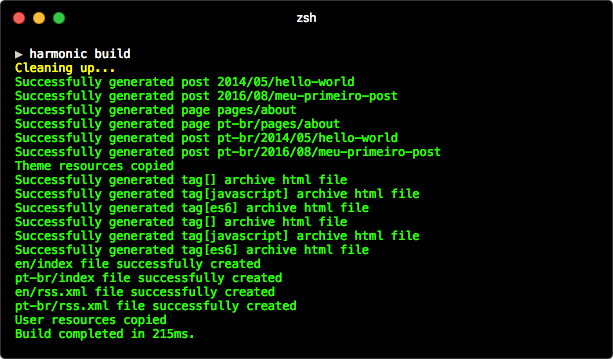
\includegraphics[width=\textwidth]{harmonic_build}
    \\Fonte: Elaborado pelo autor.
    \label{fig:comando_harmonic_build}
\end{figure}

Com estes arquivos, então, é possível abrir o arquivo \code{public/index.html} em seu navegador de preferência e navegar pelo site estático.

Note que qualquer edição ou mudança realizada nos arquivos fontes do site, incluindo edição de \textit{posts} e alteração de configurações, requer uma nova compilação para que as mudanças sejam refletidas nos arquivos compilados.

\section{Módulo de Execução do Site Estático}

O Harmonic também dispõe do comando \code{harmonic run}, que além de realizar o mesmo processo de compilação que o \code{harmonic build}, também inicia um servidor local para servir os arquivos estáticos e automaticamente abre o site estático no navegador padrão do sistema. Este é o método indicado para pre-visualização de seu site estático, pois os navegadores frequentemente bloqueiam vários recursos JavaScript ao acessar os arquivos estáticos diretamente do disco sem um servidor envolvido no processo, o que pode afetar a funcionalidade do site caso você abra os arquivos diretamente no navegador como descrito na seção anterior.

Além disso, o comando \code{harmonic run} também conta com um recurso de auto-geração de site e auto-recarregamento do navegador ("\textit{live-reload}") sempre que ocorrerem alterações nos arquivos fontes do site, assim proporcionando uma experiência de criação de conteúdos otimizada e muito mais prática e eficiente.

Por padrão, o comando \code{harmonic run} inicia um servidor local na porta \code{9356}, e abre o site no navegador padrão do sistema automaticamente. É possível customizar estes recursos, passando a porta desejada como primeiro parâmetro do comando (exemplo: \code{harmonic run 8080}), assim como desabilitar a função de abrir o site automaticamente passando a \textit{flag} \code{--no-open}.

\section{Módulo de Utilização de Temas}

Temas do Harmonic são basicamente um conjunto de arquivos HTML, escritos no sistema de \textit{templating} Nunjucks, seguindo um conjunto de regras que permitem o reuso de arquivos HTML de \textit{template} como estrutura para diferentes \textit{posts}, páginas e listagens com conteúdos diferentes. Temas comumente incluem também arquivos CSS e JavaScript, assim personalizando ainda mais o estilo e funcionalidades do site gerado.

Por padrão, sites estáticos do Harmonic são criados com o tema \code{harmonic-theme-default}. O usuário pode instalar ou criar novos temas, e selecionar qual dos temas disponíveis deve ser utilizado na geração do site estático.

% O meio padrão de distribuição de temas do Harmonic é pelo registro do npm. 
Temas do Harmonic podem ser instalados diretamente do registro de pacotes do npm, utilizando o cliente de linha de comando do npm, como pode ser visto na figura \ref{fig:comando_install_theme}.

\begin{figure}[htbp]
    \centering
    \caption{Exemplo de instalação de um tema do Harmonic.}
    \vspace{5pt}
    \lstset{language=sh}
    \begin{lstlisting}
    npm install harmonic-theme-jsrocks
    \end{lstlisting}
    Fonte: Elaborado pelo autor.
    \label{fig:comando_install_theme}
\end{figure}

É recomendável que autores de temas adicionem a palavra-chave \code{harmonictheme} ao publicar seus temas no registro de pacotes do npm, para que usuários possam encontrá-los mais facilmente utilizando o módulo de busca do npm.

Tendo o tema instalado, o usuário deve selecioná-lo para que este seja utilizado na próxima compilação do site estático. Isto pode ser feito editando o arquivo de configuração \code{harmonic.json} diretamente em um editor de texto e alterando o valor da propriedade \code{theme}, ou através do comando \code{harmonic config}.

Com a troca do tema, o estilo do site pode mudar radicalmente, como pode ser observado na figura \ref{fig:tema_jsrocks} em comparação com o tema padrão exibido na figura \ref{fig:harmonic_site_default}.

A criação de novos temas geralmente dá-se a partir da edição e personalização de um tema já existente, como o tema padrão ou qualquer outro tema disponível. %Aperfeiçoamentos no desenvolvimento de temas serão abordados na seção de trabalhos futuros no capítulo de conclusão deste trabalho.

% Embora toda a lógica de geração de sites estáticos
Vale notar que, embora o Harmonic e todos seus recursos sejam multiplataforma, compatíveis com todos os principais sistemas operacionais assim como os mais diversos conjuntos de \textit{hardware}, o que define a compatibilidade do site gerado com os navegadores e dispositivos é principalmente o tema escolhido. Os temas mantidos pela organização JS Rocks (\code{harmonic-theme-default} e \code{harmonic-theme-jsrocks}) prezam pela responsividade e compatibilidade com o maior número possível de navegadores e dispositivos, mas o mesmo não pode ser garantido para outros temas criados por terceiros.

\begin{figure}[htbp]
    \centering
    \caption{Site estático do Harmonic utilizando o tema JS Rocks.}
    \vspace{5pt}
    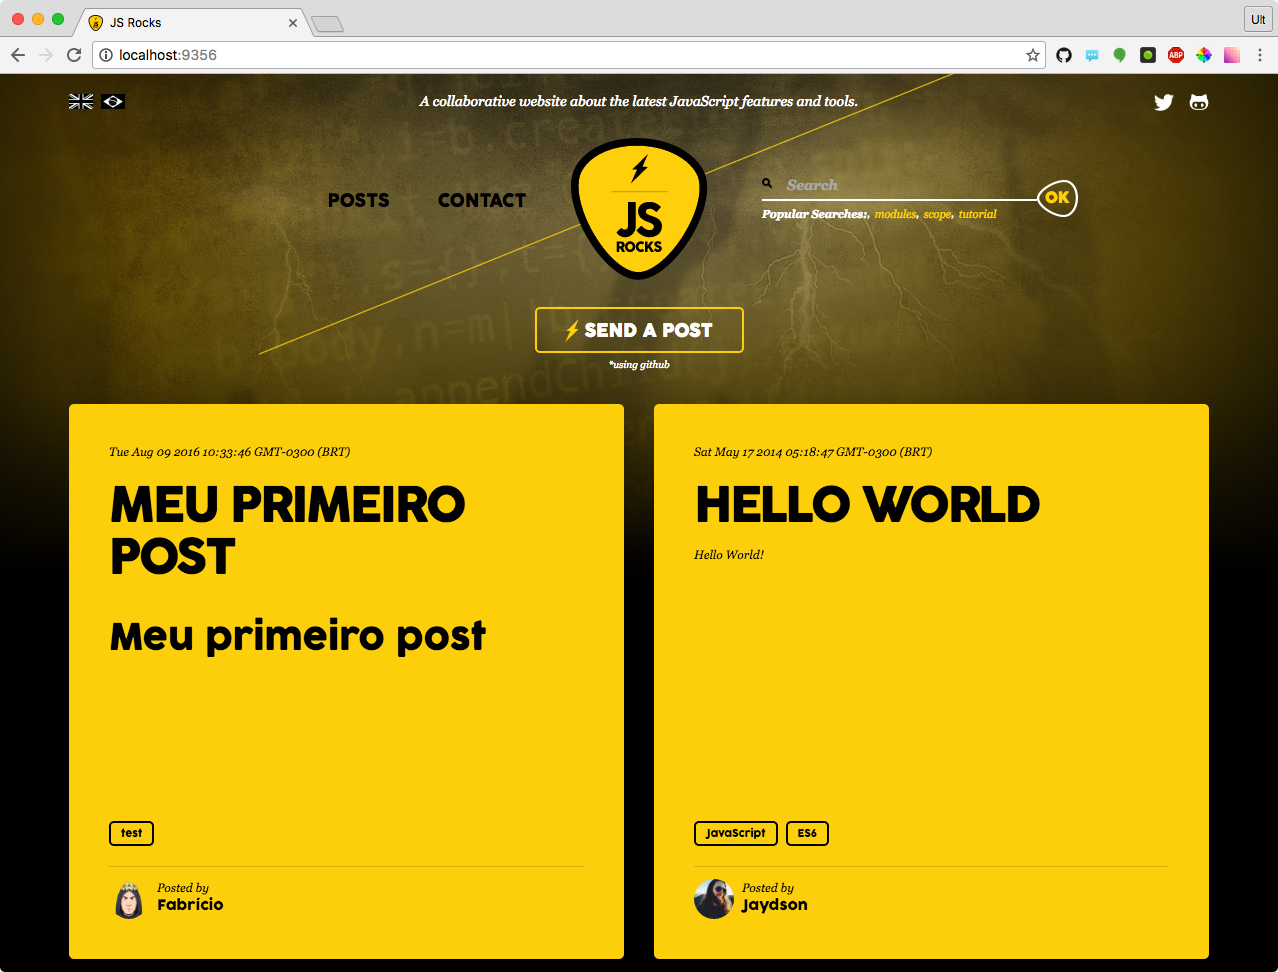
\includegraphics[width=\textwidth]{tema_jsrocks}
    \\Fonte: Elaborado pelo autor.
    \label{fig:tema_jsrocks}
\end{figure}

\section{Módulo de Ajuda}

O Harmonic, assim como praticamente toda ferramenta de linha de comando, conta com um manual do usuário que pode ser acessado através do comando \code{harmonic --help}, como pode ser visto na figura \ref{fig:harmonic_help}. % TODO consertar --

\begin{figure}[htbp]
    \centering
    \caption{Manual do Harmonic.}
    \vspace{5pt}
    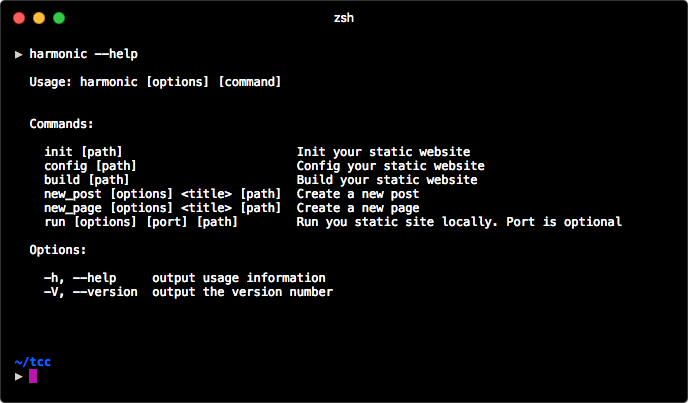
\includegraphics[width=\textwidth]{harmonic_help}
    \\Fonte: Elaborado pelo autor.
    \label{fig:harmonic_help}
\end{figure}

O Harmonic também conta com uma visão geral de sua documentação em seu repositório no GitHub, a qual pode ser acessada no endereço <\url{https://github.com/JSRocksHQ/harmonic}>, e a documentação online completa acessível no endereço <\url{https://github.com/JSRocksHQ/harmonic/tree/master/doc}>.

\section{Caso de Uso de Criação de Site Estático Simplificada}

Nesta seção será apresentado uma forma resumida de criação e execução de um site estático usando apenas os recursos principais do Harmonic.

Após ter instalado o Harmonic, o usuário pode criar um novo site estático utilizando o comando apresentado na figura \ref{fig:comando_harmonic_init}. Este comando é digitado em um programa de linha de comando, como o \textit{Command Prompt} ou \textit{Terminal}.

\begin{figure}[H]
    \centering
    \caption{Criação de um site estático pelo Harmonic.}
    \vspace{5pt}
    \lstset{language=sh}
    \begin{lstlisting}
    harmonic init
    \end{lstlisting}
    Fonte: Elaborado pelo autor.
    \label{fig:comando_harmonic_init}
\end{figure}

Este comando permite definir a configuração inicial do site estático e gera uma estrutura de arquivos e pastas que servem de base para a construção do site estático. Esta estrutura inicial já conta com uma postagem de exemplo, que pode ser editada ou excluída.

Em seguida, com a estrutura do site estático criada, o usuário pode criar novas postagens através do comando apresentado na figura \ref{fig:comando_harmonic_new_post}.

% TODO consertar acento
\begin{figure}[H]
    \centering
    \caption{Criação de uma nova postagem pelo Harmonic.}
    \vspace{5pt}
    \lstset{language=sh}
    \begin{lstlisting}
    harmonic new_post "TITULO DA POSTAGEM"
    \end{lstlisting}
    Fonte: Elaborado pelo autor.
    \label{fig:comando_harmonic_new_post}
\end{figure}

Este comando cria um arquivo Markdown para cada linguagem suportada pelo site estático, dentro da pasta \code{/src/posts/[LINGUAGEM]}, e automaticamente abre eles para edição no editor de arquivos Markdown (\code{.md}) padrão configurado no computador do usuário. Estes arquivos armazenam o conteúdo e informações relacionadas à postagem.

Em seguida, o usuário pode gerar o site e visualizá-lo em sua máquina local utilizando o comando exibido na figura \ref{fig:comando_harmonic_run}.

\begin{figure}[H]
    \centering
    \caption{Execução do site estático.}
    \vspace{5pt}
    \lstset{language=sh}
    \begin{lstlisting}
    harmonic run
    \end{lstlisting}
    Fonte: Elaborado pelo autor.
    \label{fig:comando_harmonic_run}
\end{figure}

Este comando gera os arquivos HTML, CSS e JS a partir do tema selecionado e dos arquivos fontes como \textit{posts} e configurações do site, e então automaticamente abre o site estático no navegador do usuário, como pode ser visto na figura \ref{fig:harmonic_site_default}.

\begin{figure}[H]
    \centering
    \caption{Site estático gerado pelo Harmonic com o tema padrão.}
    \vspace{5pt}
    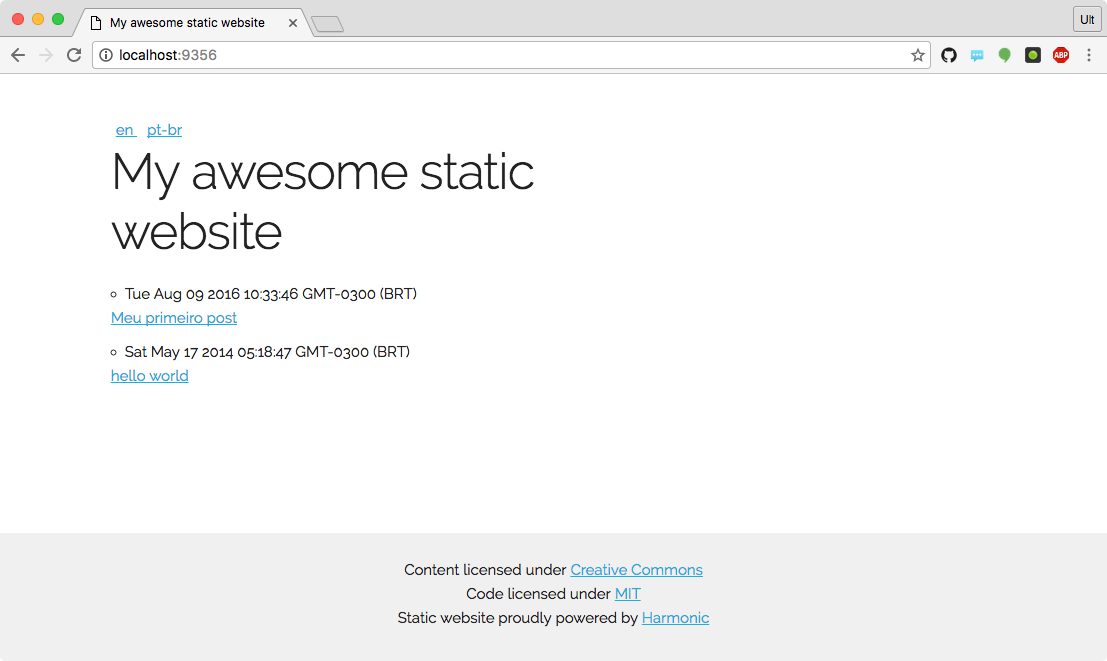
\includegraphics[width=\textwidth]{harmonic_site_default}
    Fonte: Elaborado pelo autor.
    \label{fig:harmonic_site_default}
\end{figure}

\chapter{Considerações Finais}

\vspace*{-1cm}

Nesse capítulo são resumidos os principais aspectos decorrentes do desenvolvimento deste trabalho. São discutidas os resultados obtidos e discussões, e por fim são apresentado os possíveis trabalhos futuros.

Conforme foi apresentado nesse trabalho  sistemas que gerem sites estáticos vem mostrando potencial conforme site Static Site Generators \cite{staticsitegenerators}.

O Harmonic é um projeto que pode ser instalado de forma simples e gratuita, através do gerenciador de pacotes npm. Outra característica importante é que todo seu desenvolvimento é de forma aberta e seu código fonte é acessível publicamente.

Outra contribuição importante foi o estudo com sistemas semelhantes, onde foi possível conhecer outros projetos e classificá-los levando em conta suas funcionalidades. Com isto foi possível identificar o diferencial do Harmonic, que é sua praticidade, podendo ser facilmente instalado em qualquer um dos principais sistemas operacionais (Windows, Linux, Mac), sendo assim o usuário com apenas dois comandos é capaz de criar e executar um site estático, além disso ele conta com todos os recursos essenciais para o gerenciamento do site estático sem a necessidade de configurações extras nem instalações de \textit{plugins}.

\section{Resultados Obtidos e Discussões}

Como a contribuição deste trabalho, o projeto Harmonic contempla vários propósitos, como por exemplo criar uma ferramenta de geração de sites estáticos multiplataforma, eficiente e prática. Este trabalho atende a este objetivo almejado, já que suporta os mais diversos sistemas operacionais e navegadores, bem como os mais variados \textit{hardwares}.

O outro objetivo que também foi destacado na seção 1.2 era explorar os novos recursos e funcionalidades da linguagem de programação JavaScript. O projeto Harmonic é escrito quase em sua totalidade na linguagem JavaScript, utilizando todos os novos recursos oferecidos por ela.

Como discussão o presente trabalho tem apresentado uma boa aceitação pela comunidade, tendo cerca de 150 downloads mensais, com \textit{feedback} na sua grande maioria positivo. Algumas sugestões destes usuários para melhoria deste projeto são debatidas na seção de trabalhos futuros.

\section{Trabalhos Futuros}

Dentre os aspectos para continuidade deste trabalho destaca-se: 

\subsection{Plugins}

Futuramente, desenvolvedores e usuários poderão estender as funcionalidades do Harmonic através de \textit{plugins}. A arquitetura de \textit{plugins} do Harmonic já está sendo discutida e elaborada.

Através de \textit{plugins} será possível adicionar funcionalidades completamente customizadas, como, por exemplo, buscar a foto de perfil do autor a partir de seu email usando serviços de terceiros--como o Gravatar \cite{gravatar}--, compilar arquivos durante o processo de geração do site estático cujos formatos não são suportados nativamente pelo Harmonic, criar um registro de autores para não duplicar os dados do autor nas meta-informações de cada um de seus \textit{posts}, assim como adicionar praticamente qualquer outro tipo de funcionalidade.

\subsection{Melhorias no desenvolvimento de temas}

Atualmente, a criação de um tema novo é um processo trabalhoso. A etapa de criação de tema geralmente envolve copiar o tema padrão (ou algum outro tema) e personalizá-lo até que se obtenha o tema desejado.

Estão sendo planejadas melhorias para o desenvolvimento de temas, como novos comandos para a criação de temas e aperfeiçoamento no sistema de recarregamento automático do site para tornar o desenvolvimento de temas claro e eficiente.

\subsection{Interface gráfica}

Na continuidade deste trabalho pensa-se em adicionar uma interface gráfica para uma melhor usabilidade para usuários que não estão habituados à interface de linha de comando. Com esta possibilidade, pretende-se atingir um público alvo mais abrangente.

% \chapter{Exemplo de código JavaScript}

% (capítulo temporário, por enquanto apenas testando o syntax highlighter)

% \lstset{language=JavaScript}
% \begin{lstlisting}
% // Hello.js
% function foo(arg) {
%	alert(1);
% }
% \end{lstlisting}

% Exemplo puxando o código fonte de um arquivo separado:
% \lstinputlisting[breaklines]{source.js}



\setstretch{1.0}
\nocite*
\bibliography{bibliografia}
\bibliographystyle{abnt}
\setstretch{1.5}

\chapter{Apêndices}

\section{Apêndice 1 - Requisitos Funcionais e Não-Funcionais}

Nesta seção é debatido o entendimento do domínio, os requisitos funcionais e não-funcionais, entre outros tópicos de requisitos.

\subsection{Entendimento de domínio}

Gerador de sites estáticos, construído sobre a plataforma Node.js e compatível com todos os principais sistemas operacionais (Windows, Linux, OS X).

\subsection{Requisitos funcionais}

\begin{itemize}
\item [{[RF 001]}] O sistema deve fornecer um comando para inicialização de um novo site estático, que deve criar a estrutura de pastas e arquivos necessária.
\item [{[RF 002]}] O sistema deve fornecer um comando para criação de um novo post, que deve criar um arquivo markdown com o nome desejado na pasta de posts de cada linguagem que o site suporta, contendo meta-informações básicas sobre o mesmo e o título escolhido.
\item [{[RF 003]}] O sistema deve fornecer um comando para criação de uma nova página.
\item [{[RF 004]}] O sistema deve permitir instalar novos temas.
\item [{[RF 005]}] O sistema deve permitir trocar o tema ativo, escolhendo entre os temas instalados.
\item [{[RF 006]}] O sistema deve fornecer um comando para geração do site estático a partir dos arquivos fontes (configurações, tema ativo e arquivos markdown), gerando arquivos HTML, CSS e JS como saída.
\item [{[RF 007]}] O sistema deve fornecer um comando para visualizar o site estático no computador do usuário criando um servidor local.
\item [{[RF 008]}] O sistema deve fornecer a possibilidade de atualizar o navegador automaticamente ao realizar alterações nos arquivos fonte enquanto o servidor local estiver sendo executado.
\item [{[RF 009]}] O sistema deve fornecer um comando de ajuda que explica a funcionalidade e parâmetros de todos os comandos.
\item [{[RF 010]}] O sistema deve fornecer uma forma de criar novos temas.
\item [{[RF 011]}] O sistema deve fornecer uma forma de alterar as configurações de um site já criado.
\end{itemize}

\subsection{Requisitos não-funcionais}

\begin{itemize}
\item [{[RNF 001]}] O sistema deve manter compatibilidade com todos os principais sistemas operacionais: Windows, Linux e OS X.
\item [{[RNF 002]}] O sistema deve ser desenvolvido sobre a plataforma Node.js, mantendo a compatibilidade com a versão 0.10 e versões mais recentes, como a 0.12, 4, 5 e 6.
\item [{[RNF 003]}] O sistema deve ser distribuído pelo gerenciador de pacotes npm.
\end{itemize}

\subsection{Classificação de requisitos}

\subsubsection{Gerenciamento}

\begin{itemize}
\item[\textbullet] [RF 001]
\item[\textbullet] [RF 009]
\item[\textbullet] [RF 011]
\end{itemize}

\subsubsection{Edição}

\begin{itemize}
\item[\textbullet] [RF 002]
\item[\textbullet] [RF 003]
\item[\textbullet] [RF 007]
\item[\textbullet] [RF 008]
\end{itemize}

\subsubsection{Personalização}

\begin{itemize}
\item[\textbullet] [RF 004]
\item[\textbullet] [RF 005]
\item[\textbullet] [RF 010]
\end{itemize}

\subsubsection{Publicação}

\begin{itemize}
\item[\textbullet] [RF 006]
\item[\textbullet] [RF 007]
\end{itemize}

\subsection{Dependências entre requisitos}

\begin{itemize}
\item[\textbullet] [RF 005] depende de [RF 004].
\item[\textbullet] [RF 008] depende de [RF 007].
\end{itemize}

\subsection{Resolução de conflitos}

Não existem conflitos.

\subsection{Atribuição de propriedades}

\subsubsection{Essenciais}

\begin{itemize}
\item[\textbullet] [RF 001]
\item[\textbullet] [RF 006]
\item[\textbullet] [RF 011]
\item[\textbullet] [RNF 001]
\item[\textbullet] [RNF 003]
\end{itemize}

\subsubsection{Importantes}

\begin{itemize}
\item[\textbullet] [RF 002]
\item[\textbullet] [RF 003]
\item[\textbullet] [RF 004]
\item[\textbullet] [RF 005]
\item[\textbullet] [RF 007]
\item[\textbullet] [RF 009]
\item[\textbullet] [RNF 002]
\end{itemize}

\subsubsection{Desejáveis}

\begin{itemize}
\item[\textbullet] [RF 008]
\item[\textbullet] [RF 010]
\end{itemize}

\subsection{Validação dos requisitos}

Será feito através da geração de casos de testes no intuito de desenvolver testes específicos para cada requisito.

\subsection{Gerenciamento de requisitos}

Durante o trabalho não houve alteração de requisitos.



% \chapter{Assinatura}

% \vspace{10cm}

% \begin{center}

%------------------------------------------
%\\Prof. Dr. Adenauer Corrêa Yamin\\Orientador
%\vspace{1cm}
%\\------------------------------------------
%\\Sérgio Luis Rodrigues \\Mestrando
%\end{center}


\end{document}

